\documentclass[math-font=newcm]{sjtuarticle}
\graphicspath{{figs/}}
\allowdisplaybreaks
\usepackage[style=gb7714-2015]{biblatex}
\addbibresource{ref.bib}
\usepackage{subcaption}
\usepackage{ntheorem}
\usepackage{tikz}
\usetikzlibrary{3d,perspective}
\usepackage{forest}
\usepackage[colorlinks]{hyperref}

\title{作业4}
\author{Log Creative}
\date{2024 年 5 月 16 日}
\begin{document}
\maketitle

\tableofcontents*
% \clearpage

\begin{figure}[h]
    \centering
    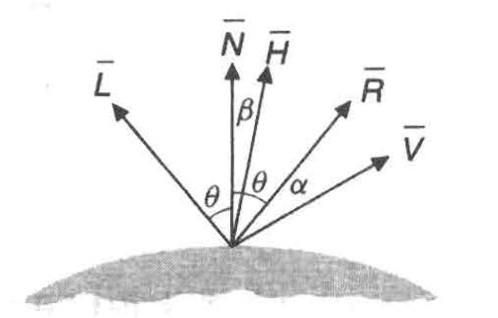
\includegraphics[width=0.5\textwidth]{angles.jpg}
    \caption{角度}
    \label{fig:angles}    
\end{figure}

\section{第1题}

使用 $(\overrightarrow{R}\cdot\overrightarrow{V})^n$ 的模型是 Phong Model,使用 $(\overrightarrow{N}\cdot\overrightarrow{H})^n$ 是 Blinn-Phong Model。Phong Model 对于反光度(shiness)较低的材质上,当 $\overrightarrow{R}$ 和 $\overrightarrow{V}$ 的夹角大于 $90^\circ$ 时,会导致高光直接变为0,也就是发生如图 \ref{fig:phong} 所示的截断现象。

\begin{figure}[h]
    \centering
    \begin{minipage}{0.45\textwidth}
        \centering
        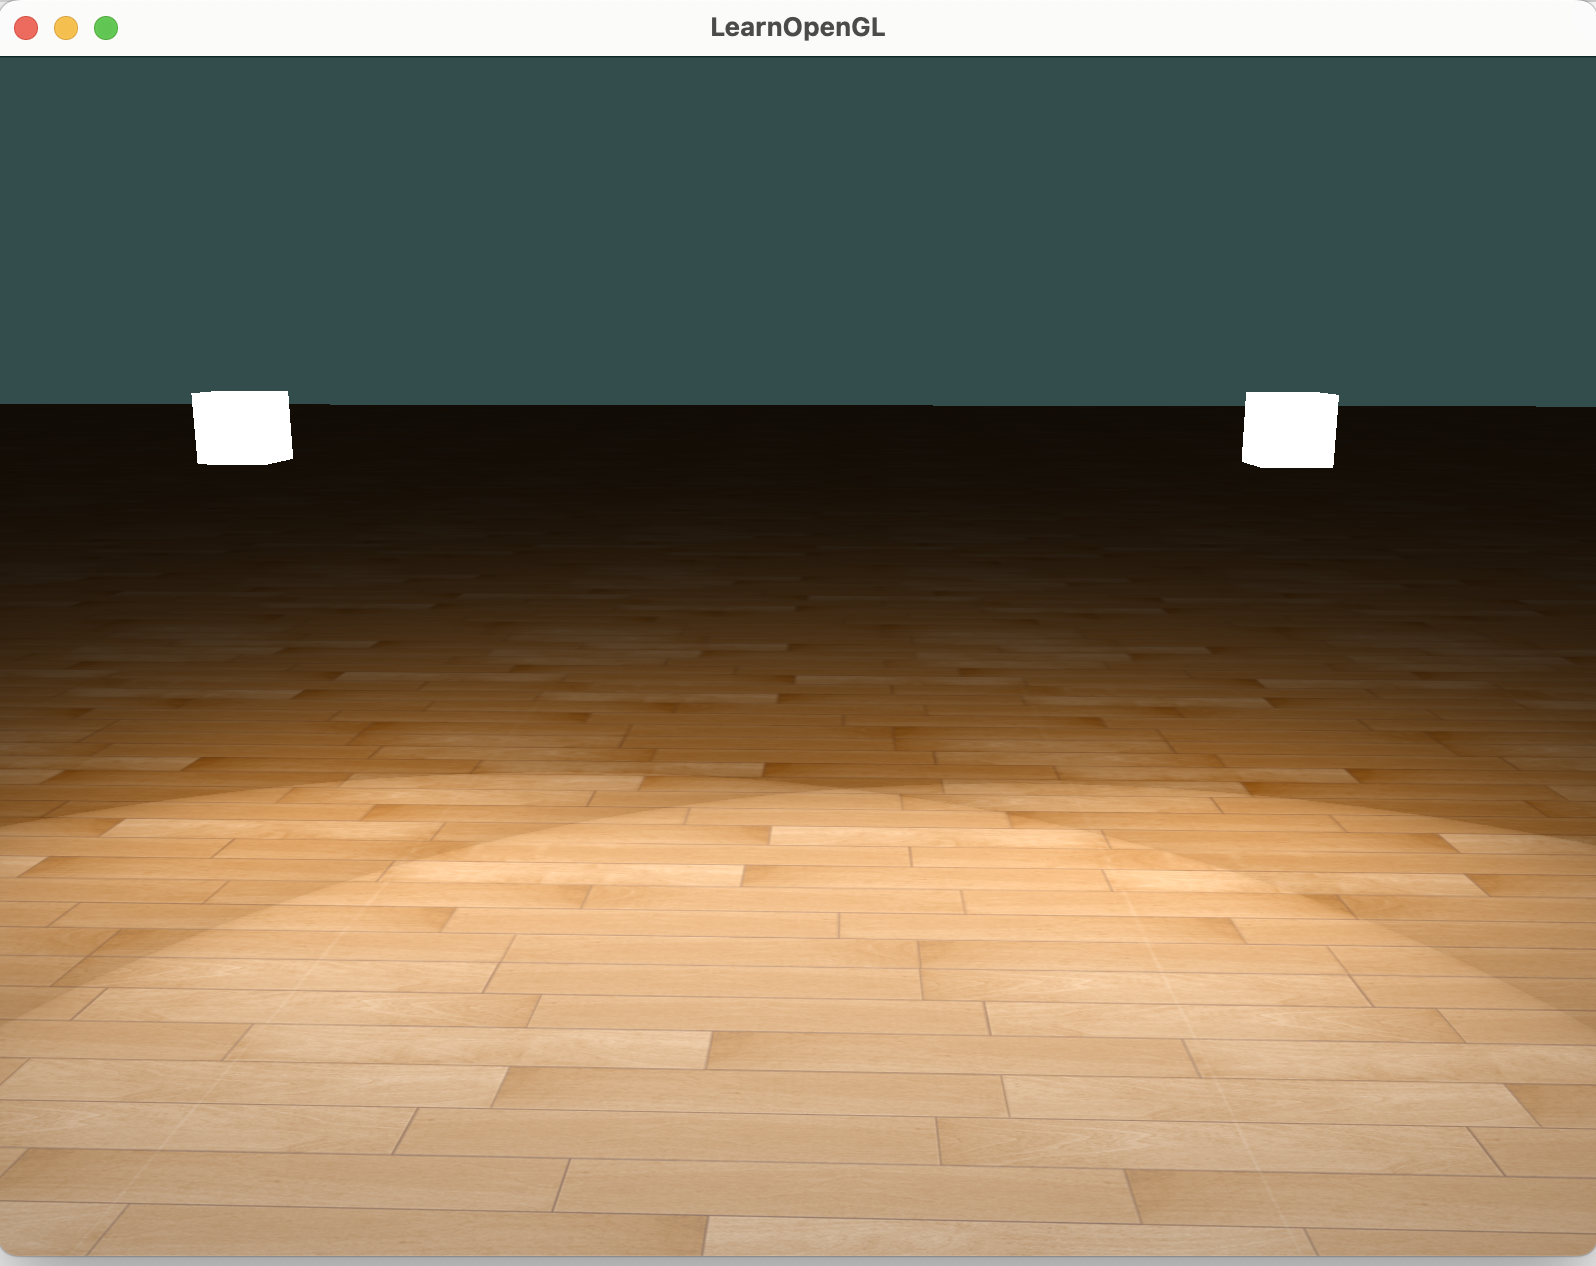
\includegraphics[width=\textwidth]{phong.png}
        \caption{Phong 模型可能导致的截断现象}
        \label{fig:phong}
    \end{minipage}
    \begin{minipage}{0.45\textwidth}
        \centering
        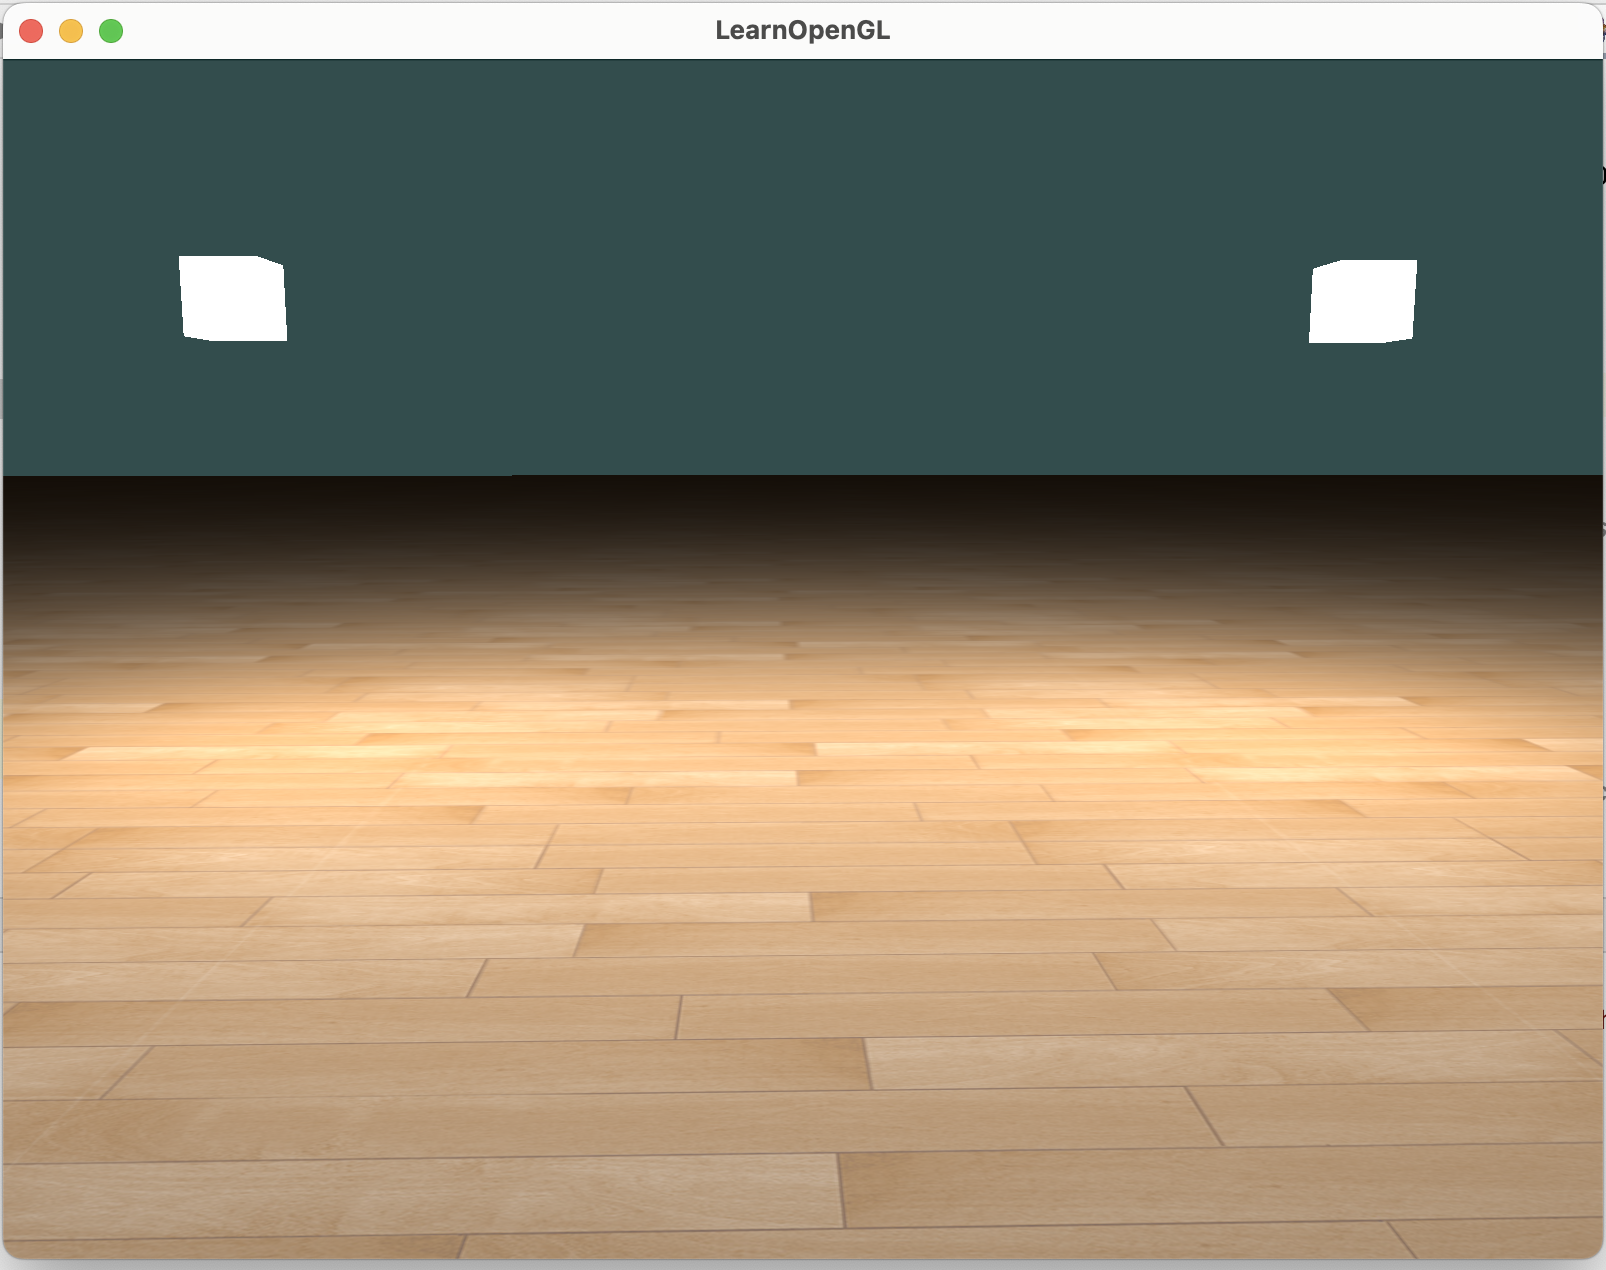
\includegraphics[width=\textwidth]{blinn-phong.png}
        \caption{Blinn-Phong 模型}
        \label{fig:blinn-phong}
    \end{minipage}
\end{figure}

而 Blinn-Phong 模型使用的是 $\overrightarrow{L}$ 和 $\overrightarrow{V}$ 的角分线 $\overrightarrow{H}$ 与 $\overrightarrow{N}$ 的角度 $\beta$ 来计算高光。现在$\overrightarrow{H}$与$\overrightarrow{N}$之间的夹角都不会超过90度(除非光源在表面以下),较好地解决了这个问题,如图 \ref{fig:blinn-phong} 所示。

\section{第2题}

\begin{proof}
    \begin{itemize}
        \item[(a)] 当所有向量共面时,由于 $\overrightarrow{H}$ 是 $\overrightarrow{L}$ 和 $\overrightarrow{V}$ 的角分线,则
        \begin{equation}\label{eq:rel}
            \theta+\beta = \theta-\beta+\alpha
        \end{equation}
        故
        \begin{equation}\label{eq:conc}
            \alpha=2\beta
        \end{equation}
        \item[(b)] 一般情况下,只能保证 $\overrightarrow{L}$、$\overrightarrow{H}$、$\overrightarrow{V}$以及 $\overrightarrow{L}$、$\overrightarrow{N}$、$\overrightarrow{R}$ 分别共面。那么 $\theta$、$\beta$、$\alpha$ 就不一定共面,式 \eqref{eq:rel} 就不一定成立,则其导出式 \eqref{eq:conc} 就不一定成立。
    \end{itemize}
\end{proof}


\end{document}